
\lettrine[lines=3]{T}{}he string interpreter is one of the significant components of plant generation. It is the final step in the process of procedural generation. The output of this stage is dependant on what the L-system is representing. In this case, it is responsible for creating the final plant models and information and then rendering it on the screen, using the OpenGL framework. 

The generation of plant-life has three main stages. The first part is the turtle graphics interpreter, then the model generator, and finally, the renderer. The turtle graphics interpreter takes the string of modules provided by the rewriter, as a set of instructions. It starts from the root of the tree and generates a skeletal structure made up of joints. This is similar to the techniques used in skeletal rigging in animation \cite{gregory2014game}. The tree skeleton joints each represent a branch segment or part of the tree. These joints have some information about the properties of that segment. The joint data is then used to generate the model data in the second stage of processing. The model generator creates the 3D points that make up the plant, as well as texture and lighting information. The models can finally be passed to the final part of the string interpreter, which is the renderer. The renderer is responsible for taking all the vertex, texture, and lighting data and renders the final plant on the screen. The renderer will also handle any physical simulation of the tree skeleton. The stages of string interpretation can be seen in figure \ref{l-system interpreter} below, as well as the information needed at each stage. 

\begin{figure}[htbp]
	{\centering
		\vspace{7px}
		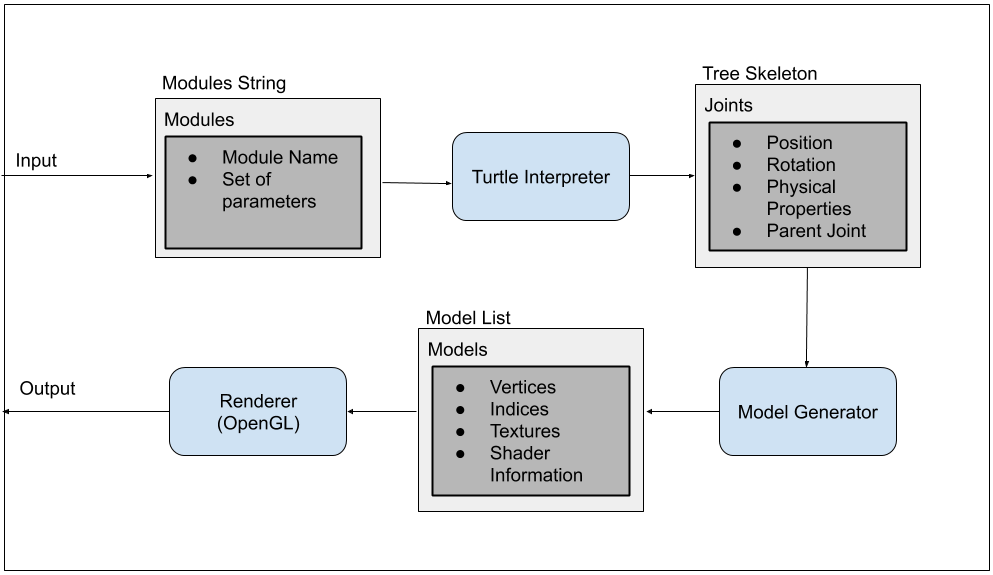
\includegraphics[scale=0.4]{Diagrams/L-systemInterpreter.png}
		\caption{Diagram of the stages of L-system interpretation and rendering} \label{l-system interpreter}
	}
\end{figure}
\FloatBarrier

\noindent
This chapter will cover each stage of the string interpreter implementation in detail. This chapter will also introduce how the interpreter can simulate and animation the plants' movements under forces such as gravity and wind in real-time. 

\section{Turtle Graphics Interpreter}

The primary purpose of the turtle graphics interpreter is to take the string of modules from the L-system rewriter and interpret each module as a turtle graphics instruction. Each instruction carries out a particular job in creating the overall structure of the plant. This stage is purely to follow the turtle graphics instructions and generate the skeletal data of the plant for the next stage.

This section is an implementation of what was covered in section \ref{Interpreting DOL-system}. Where a turtle graphics interpreter was defined for a simple DOL-system, however, there are several differences. The main difference is that the L-system string being interpreted is a parametric L-system and, therefore, consists of modules and parameters. Despite these differences, the overall concept remains the same. Each module name within the L-systems resultant string represents a particular meaning to the turtle graphics interpreter. The meaning of the module names are predefined in the string interpreter system and are dependant on what the L-system is trying to represent. The L-system defined for this thesis allows each module to provide optional parameters. These parameters may also carry particular meanings for the interpreter. For instance, the forward instruction or module name \say{F} can have three parameters. The value of the first parameter is the distance to move forward. The second and third parameter is the spring constant of the branch and the mass of the branch, respectively. These are useful in a physics simulation in order to animate the plant. 

Below is a table describing the L-system module names as well as the parameter meanings for the turtle graphics interpreter. In all of the instructions, there is also the case where no parameter is provided. This is still valid; however, if no parameter value is provided, a default value will be used.

\begin{table}[h!]
\centering
\begin{tabular}{ | c | l | l | l | l |}
\hline
	Instruction Name  & Meaning					& Parameter 1 	& Parameter 2 		& Parameter 3 \\  
\hline
\hline
	F 				&	Forward (Render)		& Length		& Spring Constant	& Branch Mass\\
\hline
	f 				&	Forward (Don't render)	& Length 		& Spring Constant	& Branch Mass\\
\hline
	+ 				&	Yaw	Right				& Angle 		&	N/A				&N/A\\
\hline
	- 				&	Yaw Left				& Angle			&	N/A				&N/A\\
\hline
	/ 				&	Pitch Up				& Angle			&	N/A				&N/A\\
\hline
	$\backslash$ 	&	Pitch Down				& Angle			&	N/A				&N/A\\
\hline
	$\land$ 		&	Roll Right				& Angle			&	N/A				&N/A\\
\hline
	\& 				&	Roll Left				& Angle 		&	N/A				&N/A\\
\hline
	! 				&	Change Width			& Branch Width	&	N/A				&N/A\\
\hline
	[ 				&	Save State				& N/A			&	N/A				&N/A\\
\hline
	] 				&	Load State				& N/A 			&	N/A				&N/A\\
\hline
\end{tabular}
\caption{Table of turtle instruction symbols and their meaning to the interpreter}
\label{instruction table 1}
\end{table}
\FloatBarrier

\noindent
Each modules' instruction is carried out one by one to generate the plants' skeletal structure. The skeleton starts without any joints at the root location. All of the rotation instructions change the current angle of the turtle, and the change width instruction changes the value of its width. When one of the forward instructions is reached, a joint is created and added to the plants' skeleton. The joints hold information about the properties of each particular segment or object of the plant. The joints properties are the position, orientation, scale, parent joint, as well as its physical characteristics. It is important to note that all of the rotation and scale transforms must happen before the forward movement. A joint holds the properties seen in the diagram below.

\begin{figure}[htbp]
	{\centering
		\vspace{7px}
		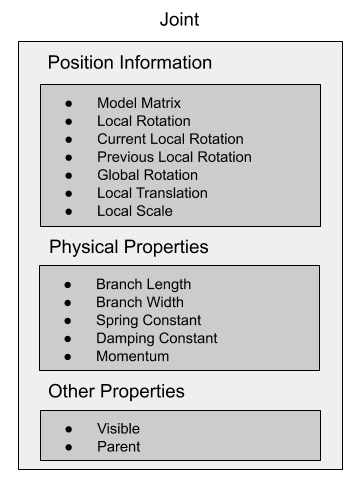
\includegraphics[scale=0.6]{Diagrams/JointDiagram.png}
		\caption{Diagram for the properties of a joint} \label{joint properties}
	}
\end{figure}
\FloatBarrier

\noindent
Figure \ref{joint properties} shows that there is a large amount of information stored for the position and orientation of each joint. This is because the rotation of the joint is stored in both a local and global space. Local space refers to the rotation of the joint relative to its parent rotation. This is useful as it allows the manipulation of subsequent child joints while leaving other joints local rotation unchanged. Global space, also known as world space, is the rotation of each joint relative to the world itself. This is useful for understanding the current rotation of the joint relative to the world. It is essential to store both the current and previous rotations as they are used to calculate the rate of change for physics calculations.

The physical properties for each joint are the parts that will affect model generation as well as physics simulations. These properties include the length, width, spring constant, damping constant as well as the current momentum of the branch. 

Take the following string of modules \say{F(1)[/(90)F(1)$\backslash$ (90)F(1)]-(90)F(1)+(90)F(1)}, the alphabet is made up of seven unique modules F, /, $\backslash$, [, ], + and -. As discussed in previous chapters the \say{F} symbol represents a move forward, and \say{+}, \say{-}, \say{/}, \say{$\backslash$} symbolize different rotations, and the \say{[} and \say{]} represent save and load state respectively. The symbols in the string above each have a single parameter except the load and save state. It is the turtle graphics interpreters' job to understand what these parameters are and how to interpret them. In this case, all of the \say{F} modules have the parameter value of 1, and all of the rotation modules have the parameter of 90. These are interpreted as the length to move forward and the change in angle from the previous joint. This interpretation can be displayed with the joint structure shown in figure \ref{skeleton diagram} below.

\begin{figure}[htbp]
	{\centering
		\vspace{7px}
		\setlength{\fboxrule}{1pt}
		\fbox{
			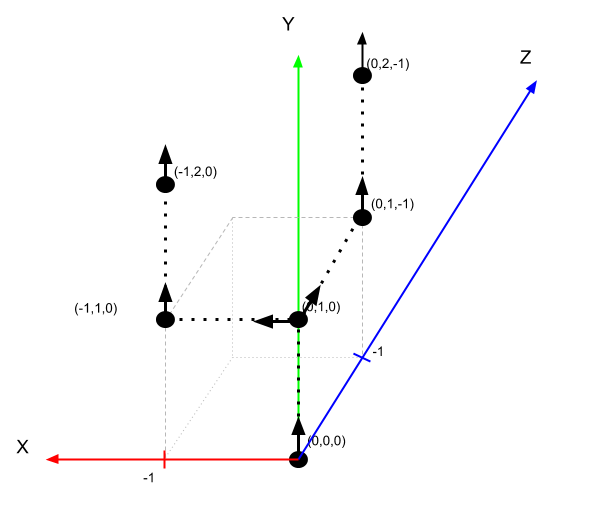
\includegraphics[scale=0.4]{Diagrams/SkeletonJoints.png}
		}
		\caption{Diagram of a simple plant skeleton with joint position and orientation.} \label{skeleton diagram}
	}
\end{figure}
\FloatBarrier

\section{Model Generator}

Modeling the branches of a plant is one of the most critical parts of the look and feel of the plant being generated. The plant skeleton and joints describe details about the plants' structure. The job of the model generator is to take the skeleton information and intelligently generate the 3D models' that make up the plants' branches, leaves, or flowers. The models of these objects are made up of vertices, normals, texture coordinates, and other low-level information that can then be provided to the OpenGL renderer and finally displayed on the screen using the GPU.

There are many different ways of procedurally modeling the branching branches of a plant. The simplest would be to take several cylinders, rotate and stack them according to each joints position in 3D space. The upside to this approach that it is very efficient, as every branch within the plant shares the same object model, which is a cylinder. This method can approximate the branching structure of the plant. However, there is a problem, which was pointed out by Baele and Warz\'{e}e ``The branches junction causes a continuity problem: to simply stack up cylinders generates a gap'' \cite{baele2005real}. The continuity problem can be seen in the figure below.

\begin{figure}[htbp]
	{\centering
		\vspace{7px}
		\setlength{\fboxrule}{1pt}
		\fbox{
			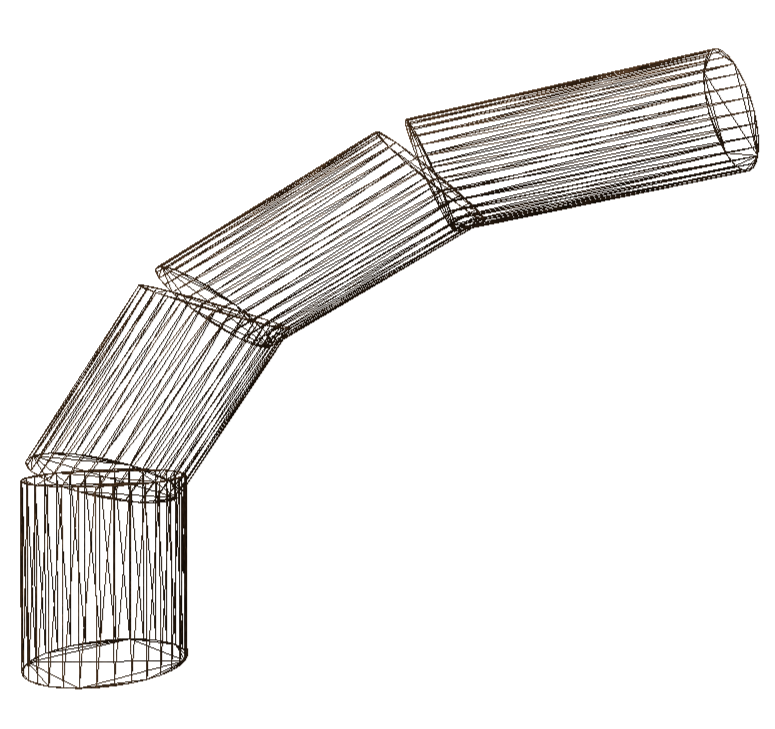
\includegraphics[scale=0.2]{Diagrams/stackedBranchesMesh.png}
		}
		\caption{Example of the continuity problem faced with stacked branching with a 25$^{\circ}$ bend per joint.}
	}
\end{figure}

\FloatBarrier

\noindent
This simple method of stacking cylinders gives a reasonable looking tree structure and it is usually good enough when the angles of branches are not more than 25$^{\circ}$ and the size of the branches do not change. However for a much more convincing tree structure there will need to be a better solution. The logical next step would be to actively link the branch segments together. This requires a number of things to take place, first of all the vertices from the previous branch top must be linked with the new top of the branch. These are the circles of vertices at either end of each branch segment. These circles will have to rotate depending on the bending direction of the branch. This means that the final model will not be made up of a large number of the same model but rather a single model with many linked branches. An example of this can be seen below:

\begin{figure}[htbp]
	{\centering
		\vspace{7px}
		\setlength{\fboxrule}{1pt}
		\fbox{
			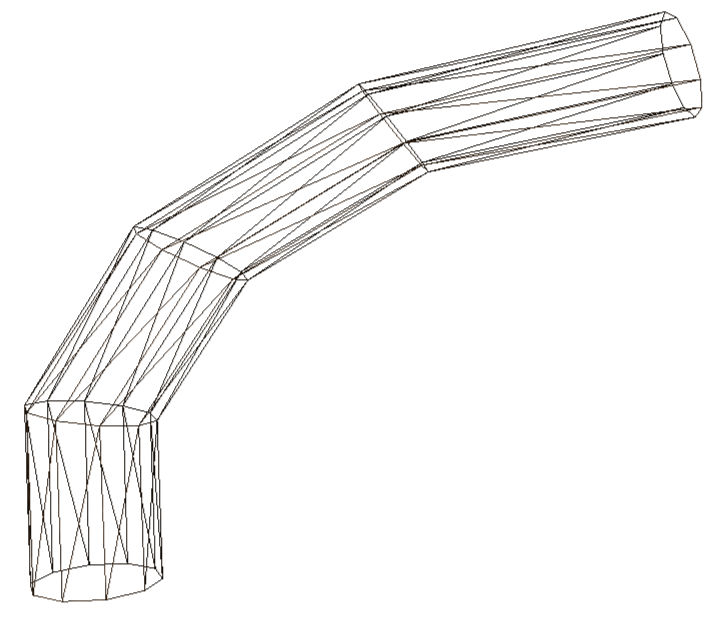
\includegraphics[scale=0.2]{Diagrams/linkedBranchesMesh.png}
		}
		\caption{Example of linked branching with a 25$^{\circ}$ bend per joint.}
	}
\end{figure}
\FloatBarrier

\noindent
This method of branch generation gives a very similar result at first glance to that of stacking cylinders. Although it does have a number of advantages, firstly it completely avoids the branch gap problem that happens with angle changes as well as branch size changes. It also means that the resolution is dynamic, meaning the number of vertices that make up a cylinder can be dynamically changed. This means that a very high resolution tree can be rendered which may look very smooth but will take a lot more computational resources, or a very low resolution tree can be rendered with more jagged edges but will require a lot less computational resources. This can be seen in figure \ref{stackedvslinked} below, where similar a looking branch can be acheived using less than half the number of vertices, with joined branches instead of stacked branches.

\begin{figure}[htbp]
	{\centering
		\vspace{7px}
		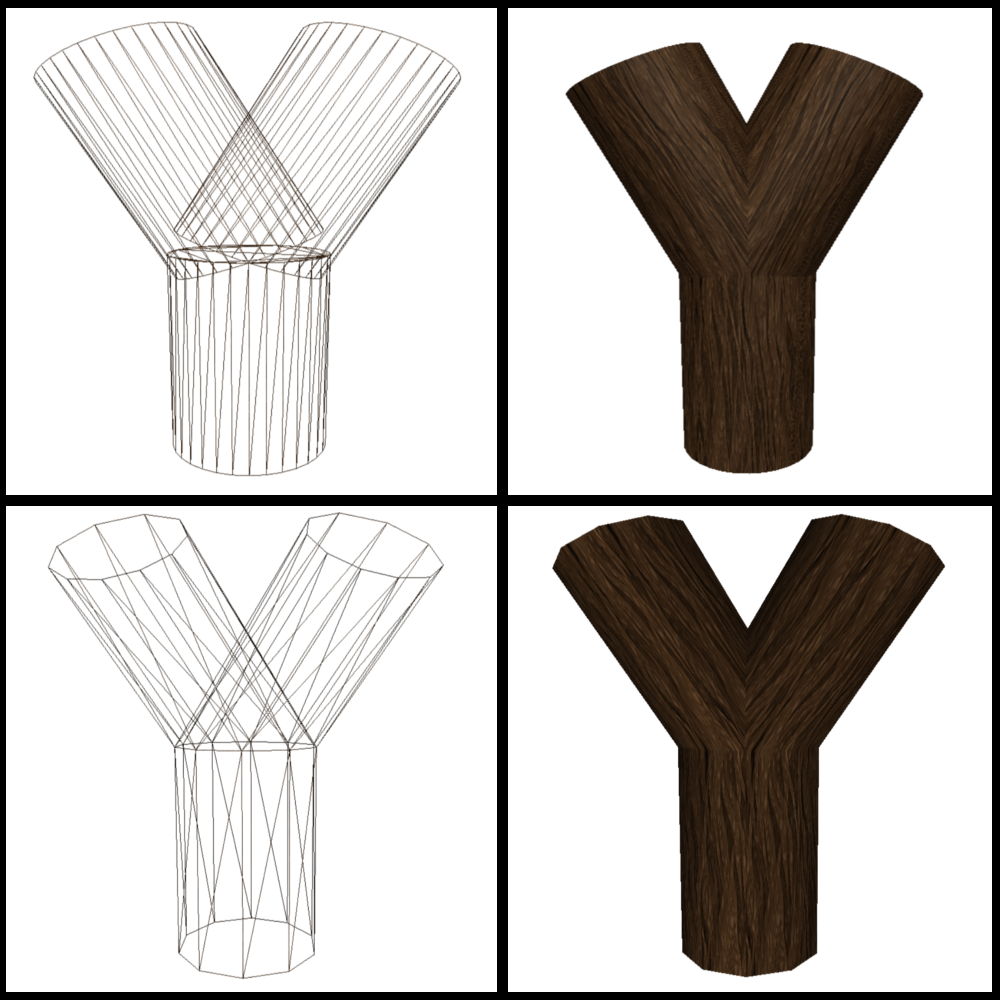
\includegraphics[scale=0.2]{Diagrams/StackedVsLinked.png}\label{stackedvslinked}
		\caption{Stacked Vs Linked.}
	}
\end{figure}
\FloatBarrier



\section{Renderer}

\noindent
The renderer is the final stage in the procedural generation pipeline. It takes all of the 3D models generated by the model generator, such as leaves, branches and flowers and renders them on the screen.  For this thesis, the \acrlong{opengl} (\acrshort{opengl}) application programming interface is use used to efficiently render the models on the screen using the \acrlong{gpu} (\acrshort{gpu}). 

The \acrshort{gpu} is a specially designed piece of harware for processing computer graphics and image processing, it has hundereds or even thousands of individual compute cores which can be used in parallel. Due to the highly parallel nature of the \acrshort{gpu}, the \acrshort{opengl} framework helps to abstract the hardware and create an interface to interact with the \acrshort{gpu} in a simpler way. There are a number of other types of graphics \acrshort{api} such as Vulkan, Metal or DirectX. These \acrshort{api}s all provide a way of interacting with the hardware behind the scenes, However, they each have a different approach. Therefore, this section will not be be going into great detail about about the specifics of \acrshort{opengl} but rather the general concepts required for rendering the plant model on the screen. The main parts of the rendering stage has to do with how model data is stored into buffer objects, secondly how textures are stored and then mapped to a certain object and thirdly how lighting can be calculated for a procedurally generated object.

\subsection{Models and Buffer Objects}

The model generator produces all of the information neccessary for the renderer to produce the result on the screen. In general the model data will consist of vertex data, texture co-ordinates and vertex normals. The vertex data is simply position of a point within a model, three vertices make up a face and the faces are what are ultimately rendered on the screen. The texture co-ordinates are the locations on a texture image which maps directly to the model vertices. Finally the vertex normals simply known as normals are the average normal vector. A normal vector being the vector that is purpendicular to the surface at a given point, and can be used for Phong shading or other types of lighting techniques.  

One of the most important parts of the rendering process is buffering the model data onto the \acrshort{gpu}. The \acrlong{vbo} (\acrshort{vbo}) is a data structure within the \acrshort{opengl} library which can be used to store this data on the \acrshort{gpu}. Generally, the data is stored as a single buffer or array with the first 3 values being a vertex position, the second two being a texture co-ordinate and the last three being a vertex normal. 

\begin{figure}[htbp]
	{\centering
		\vspace{7px}
		\setlength{\fboxrule}{1pt}
		\fbox{
			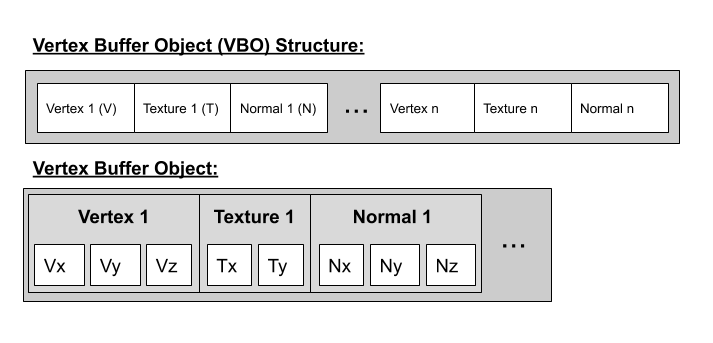
\includegraphics[scale=0.5]{Diagrams/VertexObjects.png}
		}
		\caption{Diagram showing the structure of a vertex buffer object.}
	}
\end{figure}
\FloatBarrier

Buffer objects can be created not only for the plant as a whole but potentially for different parts of the plant. For instance, the leaves on the tree are all quite similar. There is no need to have thousands of copies of a leafs vertices and textures. This would be highly wasteful and unnecessary. Simply, there could be one copy of the vertex data and texture data and instanced renderering can be used to render many copies of this object in at different places in one scene. 

\section{Shaders}

\section{Summary}








